\documentclass{beamer}
\usetheme[pageofpages=of,% String used between the current page and the
                         % total page count.
          bullet=circle,% Use circles instead of squares for bullets.
          titleline=true,% Show a line below the frame title.
          alternativetitlepage=true,% Use the fancy title page.
       %   titlepagelogo=logo-polito,% Logo for the first page.
       %   watermark=watermark-polito,% Watermark used in every page.
       %   watermarkheight=100px,% Height of the watermark.
       %   watermarkheightmult=4,% The watermark image is 4 times bigger
                                % than watermarkheight.
          ]{Torino}

\setbeamertemplate{footline}{
  \begin{beamercolorbox}[wd=\paperwidth,ht=1ex,dp=1ex]{footline}
    \vspace{5pt} \hspace{1em} \insertframenumber/\inserttotalframenumber
  \end{beamercolorbox}
}

\author{Brendon J. Brewer}
\title{STATS 331 -- Introduction to Bayesian Statistics}
\institute{The University of Auckland}
\date{}


\linespread{1.3}
\usepackage{minted}
\usepackage[utf8]{inputenc}
\usepackage{dsfont}
\newcommand{\given}{\,|\,}
\newcommand{\balpha}{\boldsymbol{\alpha}}
\newcommand{\bmu}{\boldsymbol{\mu}}


\begin{document}

\frame{\titlepage}

\begin{frame}
\begin{center}
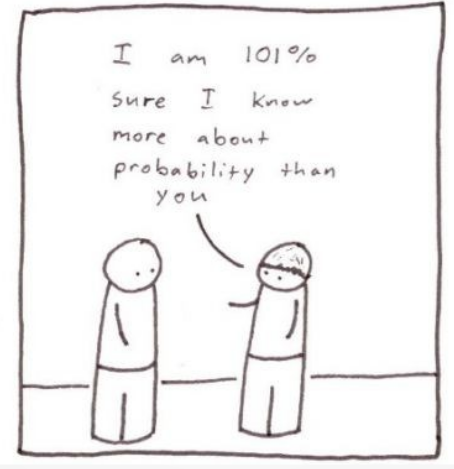
\includegraphics[width=0.6\textwidth]{images/101.png}

Credit: www.afewpanels.com
\end{center}

\end{frame}


\begin{frame}
\Large

\begin{center}
Time Series Models
\end{center}
\end{frame}

\begin{frame}
\frametitle{Poll}
How many of you have studied a course involving `time series models'
such as the AR(1)?
\end{frame}


\begin{frame}
\frametitle{What is a Time Series}
There are two related meanings for the term {\bf time series}.

\begin{itemize}
\item [(1)] Any quantity that varies over time.
\end{itemize}

\begin{center}
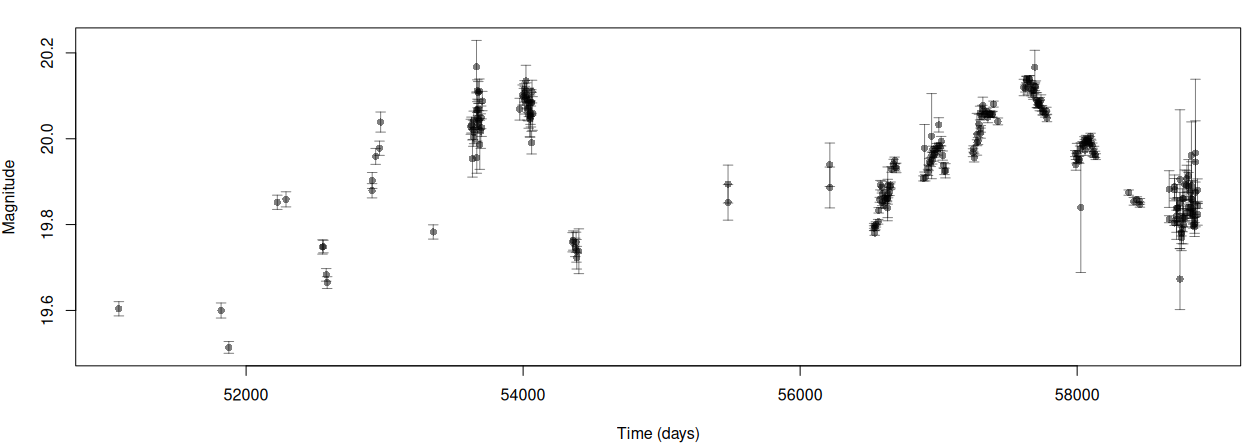
\includegraphics[width=0.9\textwidth]{images/time_series.png}
\end{center}

\end{frame}

\begin{frame}
\frametitle{What is a Time Series}
There are two related meanings for the term {\bf time series}.

\begin{itemize}
\item [(2)] A {\bf probability distribution} for a quantity that varies over time.\pause
\item That is, not any single curve, but a probability distribution over the
set of possible curves.
\end{itemize}

\end{frame}


\begin{frame}
\frametitle{Time Series Models}
Time series models are heavily used in finance, but are also used in a 
variety of other fields (e.g., the previous plot was astronomy data).

\end{frame}

\begin{frame}
\frametitle{The AR(1) Model}

\begin{itemize}
\item In STATS 331 we will only study the AR(1) model, which is a relatively simple
time series model. The AR stands for auto-regressive.\pause
\item It is a probability distribution for the values $y_1, y_2, y_3, ...$
of a series at times $t=1, 2, ...$.
Time is {\bf discrete} and there are {\bf no gaps}.\pause
\item Remember, no single curve $(y_1, y_2, y_3, ...)$ is an AR(1), it is
the probability distribution for the curve that is AR(1).\pause
\item The AR(1) might be a prior distribution or a sampling distribution
depending on the application. For us, it will be the latter.
\end{itemize}
\end{frame}

\begin{frame}
\frametitle{The AR(1) Model}

\begin{itemize}
\item The value of the quantity $y_{t+1}$ at the next timestep is given by
a function of the current value $y_{t}$ plus an `innovation'.\pause
\item We only specify a probability distribution for the innovations.\pause
\end{itemize}
\begin{align}
y_{t+1} &= \mu + \alpha(y_t - \mu) + \epsilon_t \\
\epsilon_t \given \beta &\sim \textnormal{Normal}(0, \beta^2).
\end{align}

\end{frame}


\begin{frame}
\frametitle{The AR(1) Model: Parameters}
In the previous equations we introduced the
three parameters of the AR(1) model:\pause
\begin{itemize}
\item $\mu$ describes the mean level that the $y$s fluctuate around.\pause
\item $\alpha$ describes how strongly the next value $y_{t+1}$ is influenced
by the current value $y_t$. It is usually between 0 and 1.\pause
\item $\beta$ describes the typical size of the innovations.
\end{itemize}

\end{frame}


\begin{frame}
\frametitle{Thinking About the AR(1)}
If we set $\beta$ to zero, the AR(1) process becomes deterministic and
describes an exponential decay towards $\mu$. The speed of the decay is
controlled by $\alpha$.
\begin{align}
y_{t+1} &= \mu + \alpha(y_t - \mu)
\end{align}

\end{frame}


\begin{frame}[fragile]
\frametitle{Simulating an AR(1) in R}
\begin{minted}{r}
N = 1000       # Length of simulation
mu = 5.0       # Parameters
alpha = 0.99
beta = 1
y = numeric(N) # Storage
for(i in 1:(N-1))
{
    y[i+1] = mu + alpha*(y[i] - mu) + beta*rnorm(1)
}
\end{minted}

\end{frame}

\begin{frame}[fragile]
\frametitle{Simulating an AR(1) in R}
\begin{center}
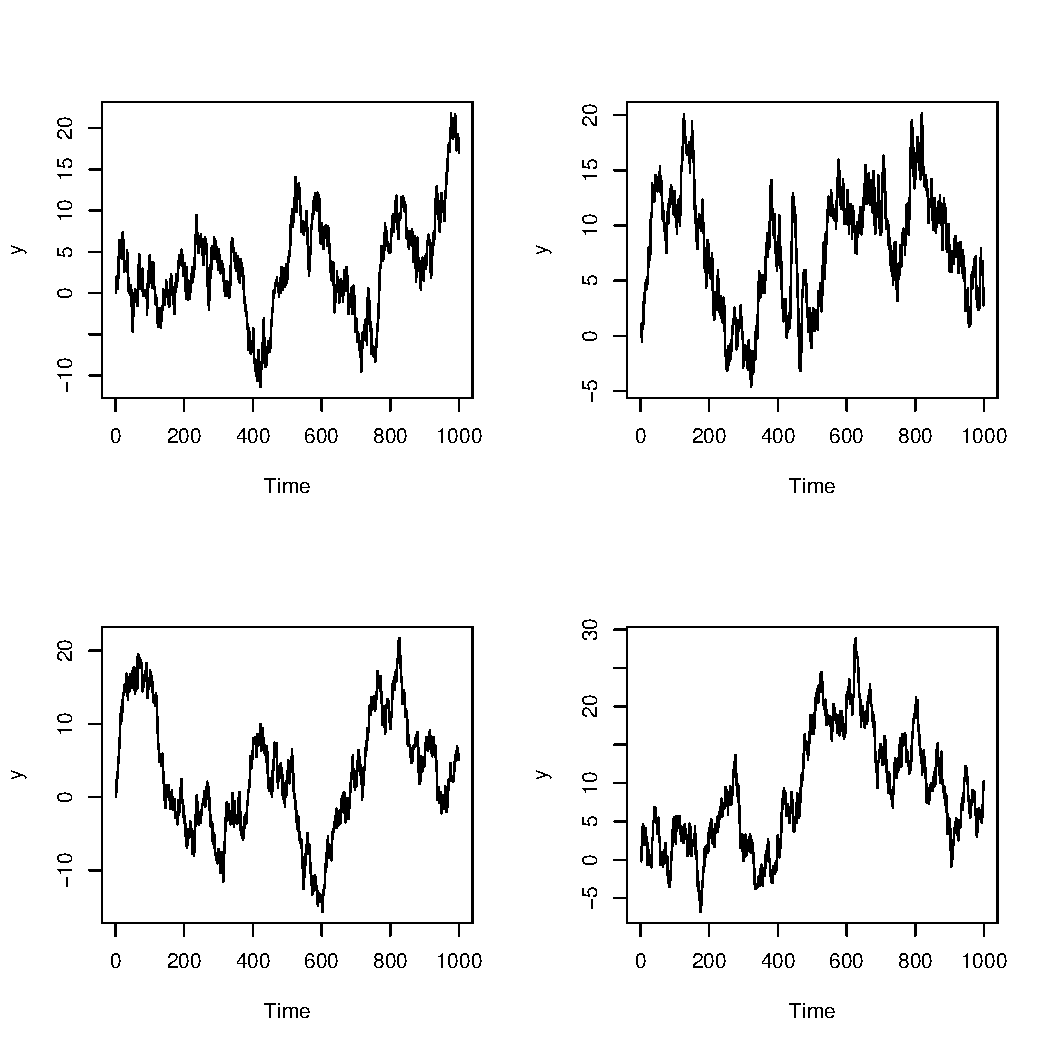
\includegraphics[width=0.6\textwidth]{images/ar1.pdf}
\end{center}

\end{frame}


\begin{frame}[fragile]
\frametitle{Mystery Data}
\begin{center}
\includegraphics[width=0.6\textwidth]{images/nzd.pdf}
\end{center}

\end{frame}

\begin{frame}[fragile]
\frametitle{Mystery Data}
The data is not actually mysterious --- it's the NZD/USD exchange rate
every day from some time in 2018 to some time in 2025.
We can `fit an AR(1) model' (i.e., infer the three parameters)
and then use that to make predictions.
\end{frame}


\begin{frame}[fragile]
\frametitle{The $\alpha$ Parameter}
The $\alpha$ parameter is quite difficult to interpret and therefore to assign
a prior distribution to. Values close to 1 make the autocorrelation high and
values close to 0 make it low, but 0.99 and 0.999 are quite different from
each other.\\\pause

It is more convenient to work with
\begin{align}
L &= -\frac{1}{\log(\alpha)}
\end{align}
which describes the autocorrelation timescale.
The inverse is $\alpha = e^{-1/L}$.

\end{frame}

\begin{frame}[fragile]
\frametitle{Priors}
Let's use simple priors for the three parameters.
\begin{minted}{r}
mu ~ dunif(-1000, 1000)
log_L ~ dunif(-10, 10)
L <- exp(log_L)
alpha <- exp(-1/L)
log_beta ~ dunif(-10, 10)
beta <- exp(log_beta)
\end{minted}

\end{frame}

\begin{frame}[fragile]
\frametitle{Sampling Distribution}
The sampling distribution/likelihood part of the model is slightly awkward,
because when we wrote down the definition of the AR(1) we did not write down
a probability distribution for the first point, $y_1$, given the parameters.
We have two options:\pause
\begin{itemize}
\item Write down $p(y_1 \given \mu, \alpha, \beta)$, possibly using an
assumption of `stationarity'.\pause
\item Treat $y_1$ as prior information instead of data, so just treat
$y_2, y_3, ..., y_N$ as the data.\pause
\end{itemize}
We will take the second approach.

\end{frame}


\begin{frame}[fragile]
\frametitle{Sampling Distribution}
Here is the code. Notice how closely it resembles the R code for simulating
data!

\begin{minted}{r}
for(i in 1:(length(y) - 1))
{
    y[i+1] ~ dnorm(mu + alpha*(y[i] - mu), 1/beta^2)
}
\end{minted}

\end{frame}

\begin{frame}[fragile]
\frametitle{Results}
Let's run JAGS and look at:

\begin{itemize}
\item The trace plots.\pause
\item The marginal posterior for $\mu$.\pause
\item The joint posterior for $\mu$ and $\log(L)$.
\end{itemize}

\end{frame}



\begin{frame}[fragile]
\frametitle{Joint Posterior}
\begin{center}
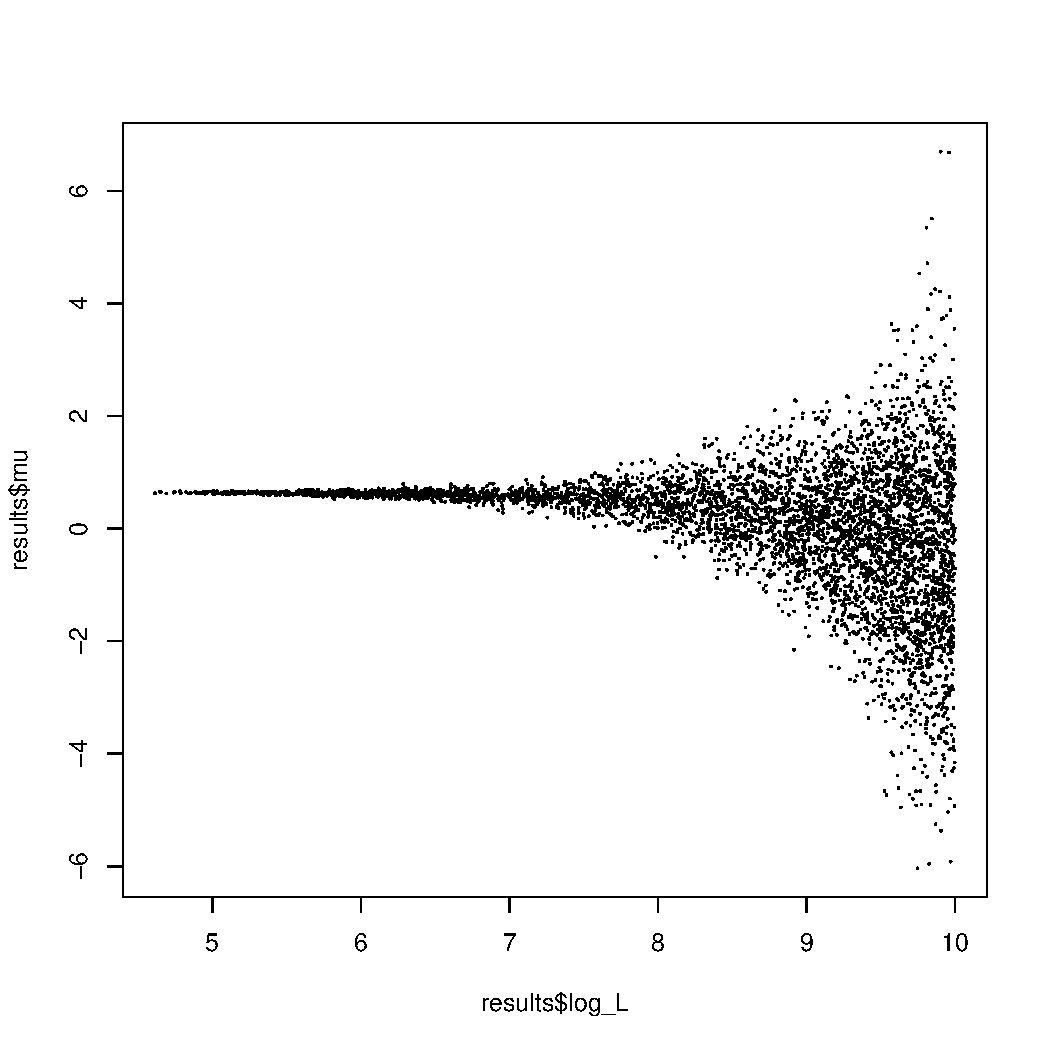
\includegraphics[width=0.6\textwidth]{images/nzd_posterior1.pdf}
\end{center}

\end{frame}


\begin{frame}[fragile]
\frametitle{Results}
Why do we get such a strong dependence in the posterior between
$\mu$ and $\log(L)$?\\[0.5em]\pause

It's because the data {\em could} be explained as being a very small piece
of a process with a very long timescale and a $\mu$ value that is very far
from the current value. Maybe the NZD `gravitates towards' 10 USD but we
just have to wait thousands of years to see it!
\end{frame}


\begin{frame}[fragile]
\frametitle{Informative Prior}
We can  with the posterior distribution by using an
informative prior. Something like this might seem reasonable:
\begin{minted}{r}
mu ~ dt(0.7, 1/0.2^2, 4)T(0, )
\end{minted}
\pause

I am showing you a new feature --- the \mintinline{r}{T(0, )} will put
some {\bf truncation} at zero so $\mu$ can't go negative. Upper limits can also
be specified, but we didn't here.
\end{frame}



\begin{frame}[fragile]
\frametitle{Joint Posterior}
\begin{center}
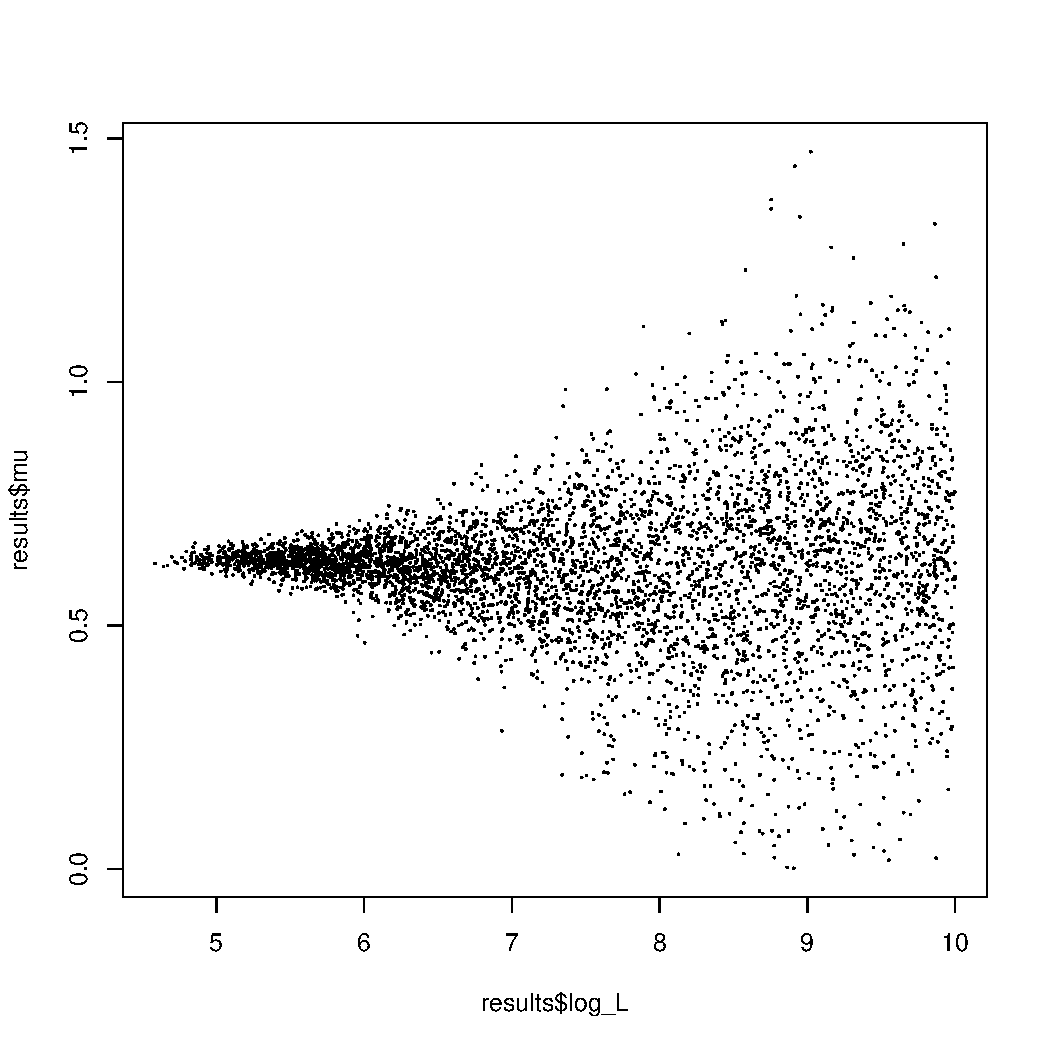
\includegraphics[width=0.6\textwidth]{images/nzd_posterior2.pdf}
\end{center}

\end{frame}

\begin{frame}[fragile]
\frametitle{Informative Prior}

\begin{itemize}
\item The informative prior might not be appropriate.
Knowledge of the typical value around which the
NZD gravitates is based on the data itself, not any external/prior information.\pause
\item One could argue back, that we have information from further in the past,
or from the behaviour of similar currencies,
that might justify the informative prior.
\end{itemize}


\end{frame}


\begin{frame}[fragile]
\frametitle{Predicting the Future}

To predict the future, we use the same procedure as we have done before:
adding new nodes which look like more data points (but are unobserved).\\[0.5em]

This is slightly more difficult for the AR(1) model than for previous models.

\end{frame}



\begin{frame}[fragile]
\frametitle{Predicting the Future}

\begin{minted}{r}
y_new[1] <- y[length(y)]
for(i in 1:365)
{
    y_new[i+1] ~ dnorm(mu + alpha*(y_new[i] - mu),
                       1/beta^2)
}
\end{minted}


\end{frame}

\begin{frame}[fragile]
\frametitle{Predicting the Future: Plotting Code}

\begin{minted}{r}
# I only monitored y_new
results = as.matrix(results) # So a row is a vector
t = seq(length(data$y), length(data$y) + 365)
plot(data$y, type="l", xlab="Time",
     xlim=c(0, max(t)), ylim=c(0.3, 0.9))
rows = sample(1:nrow(results), 10)
for(row in rows)
    lines(t, results[row, ], col=rgb(0, 0, 0, 0.3))
\end{minted}


\end{frame}



\begin{frame}[fragile]
\frametitle{Prediction}
\begin{center}
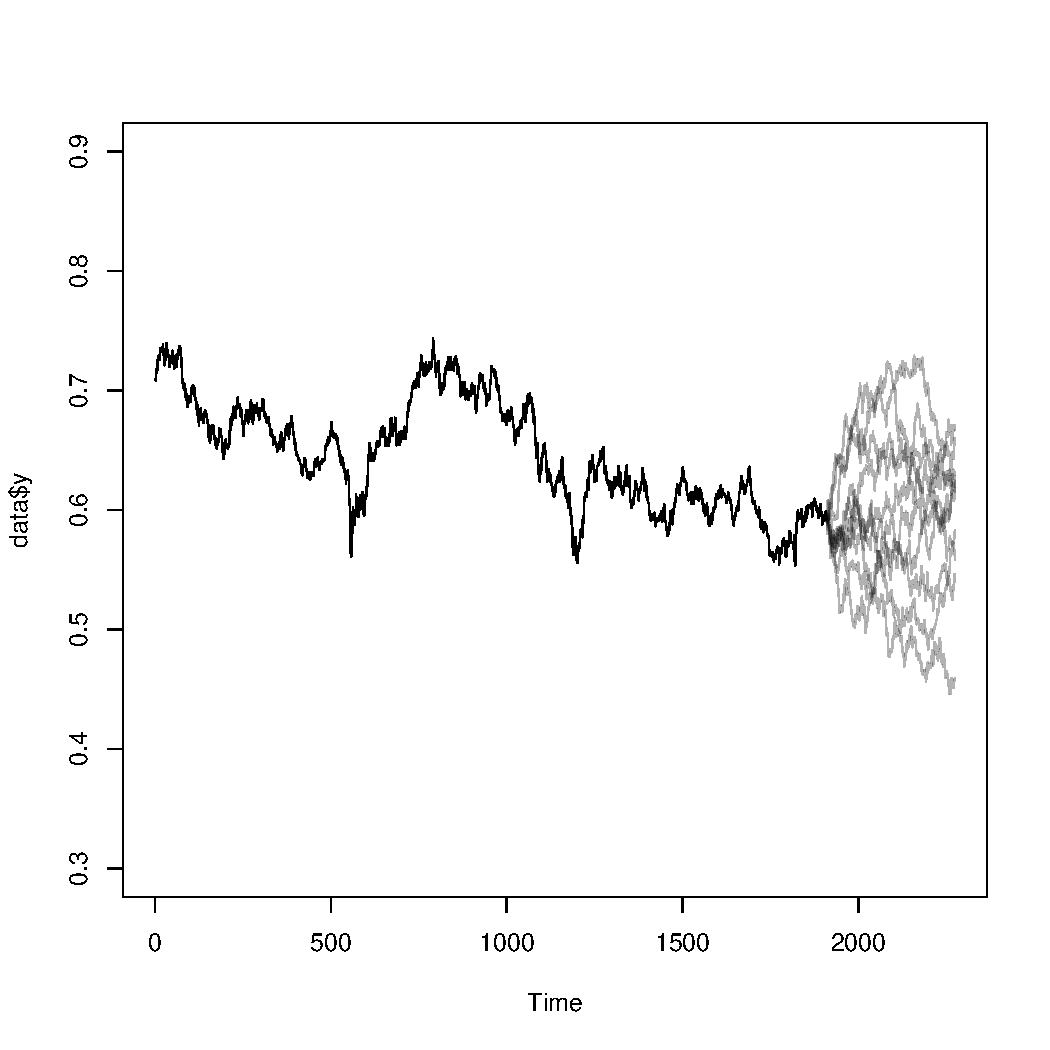
\includegraphics[width=0.6\textwidth]{images/nzd_prediction.pdf}
\end{center}

\end{frame}



\begin{frame}[fragile]
\frametitle{Prediction}
We can also make a one year forecast by looking at the posterior
distribution for \mintinline{r}{y_new[366]}.

\end{frame}

\begin{frame}[fragile]
\frametitle{Disclaimer}

\begin{itemize}
\item I like this example, but simplistic models of financial
things can cause trouble in the real world!\pause
\item The AR(1) model makes quite strong assumptions about
what is likely to happen long term, and doesn't know
anything about what causes prices (supply/demand etc).
\end{itemize}

\end{frame}


\begin{frame}
\frametitle{Conclusion}

\begin{itemize}
\item We looked at one relatively simple time series model, the AR(1).\pause
\item It is just a probability distribution for a collection of values,
and can be used as a prior or as a sampling distribution, depending on what's
appropriate for the situation at hand.\pause
\item The Bayesian framework for inferring parameters and making predictions
works just as it usually does.
\end{itemize}

\end{frame}


\end{document}

